
\section{Event Reconstruction and Selection }
\label{sec:reco}

Signals from each detector is recorded by the CAEN V1742 digitizer at $0.2$~ns time intervals.
The baseline pedestal for each channel is determined using the time samples outside of
the signal window, and is subsequently subtracted from the signal pulses. Examples of recorded
signal waveforms in the CdTe sensor for electromagnetic showers are shown in Figure~\ref{fig:Pulses}.
Using randomly triggered data, we measured the RMS of the noise for the channel reading out 
the CdTe sensor to be about $1.2-1.3$~mV. 

%Fig: Pulse shapes for various energies
\begin{figure}[htbp] 
\centering
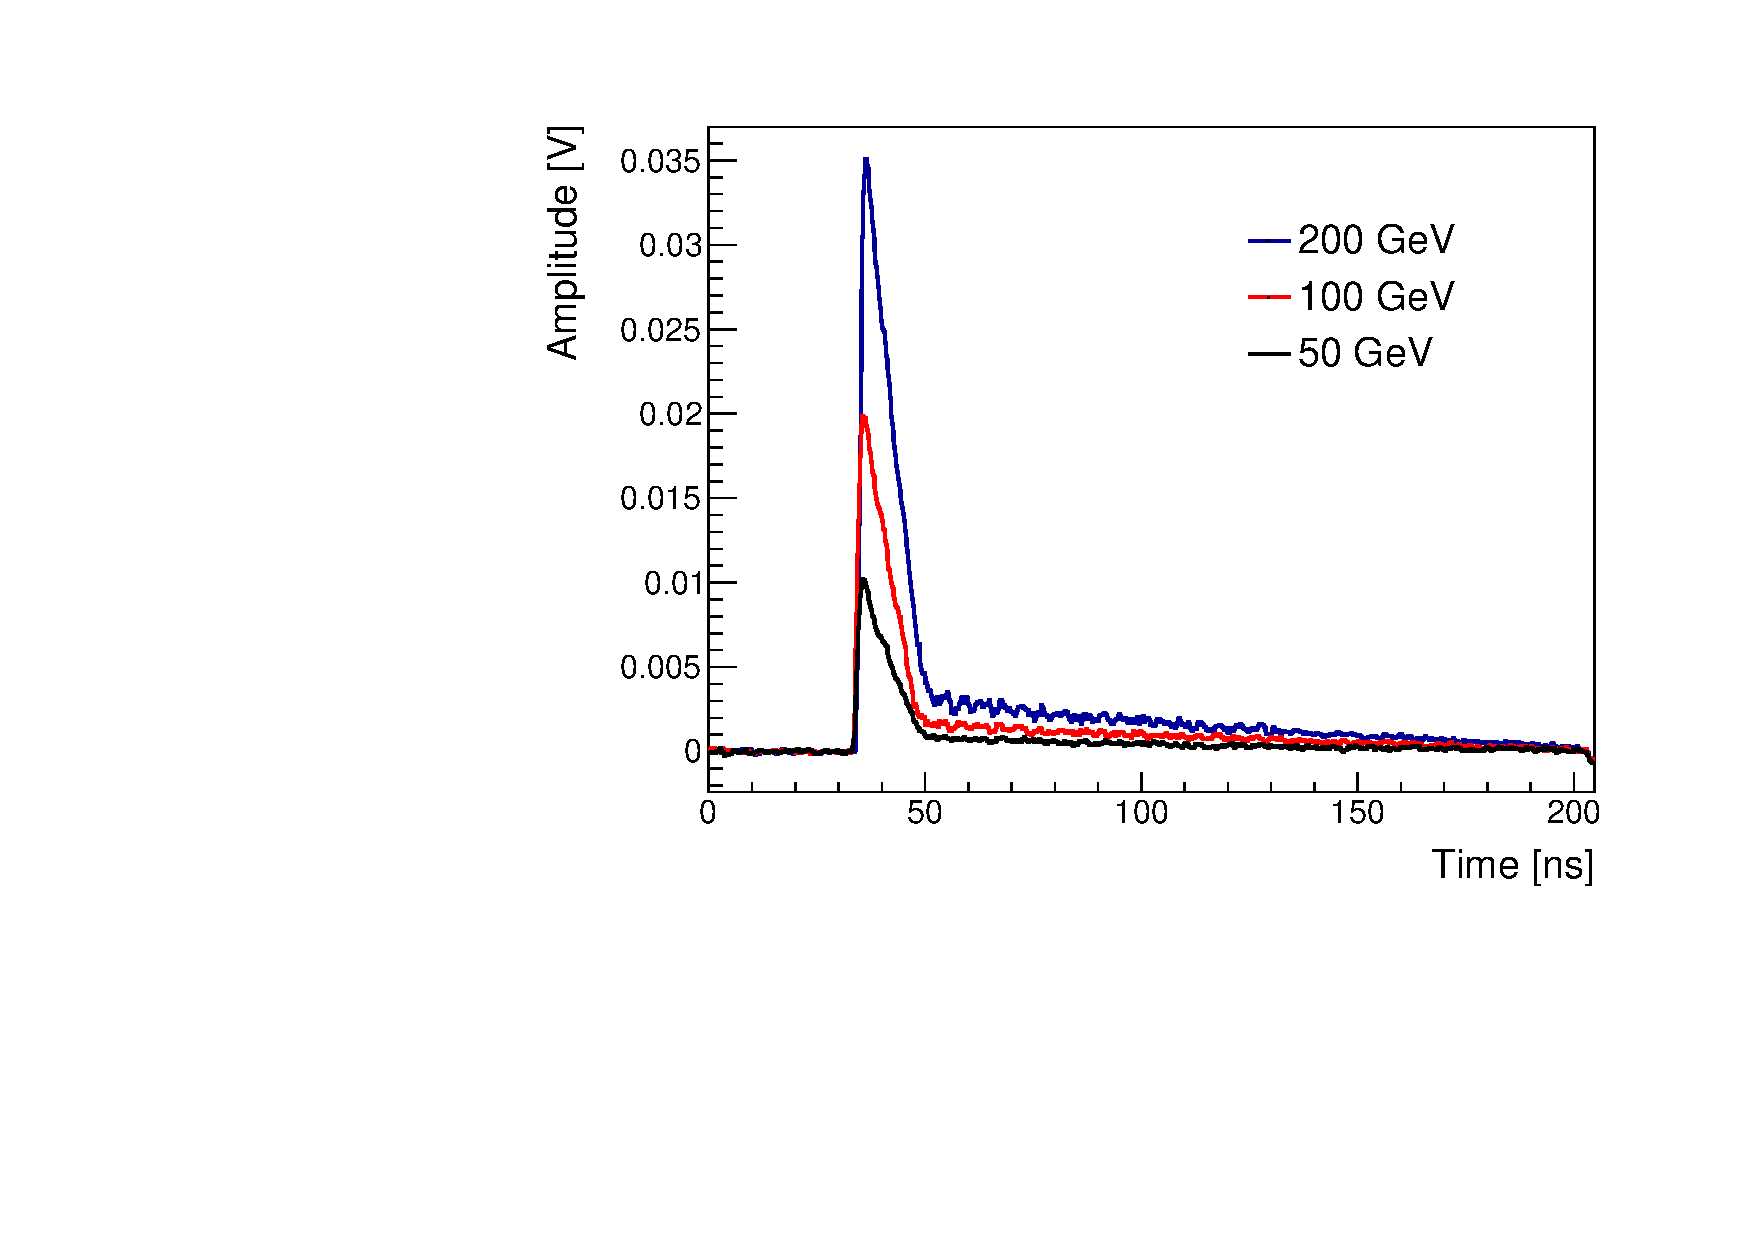
\includegraphics[width=0.49\textwidth]{figures/TypicalPulses.pdf}
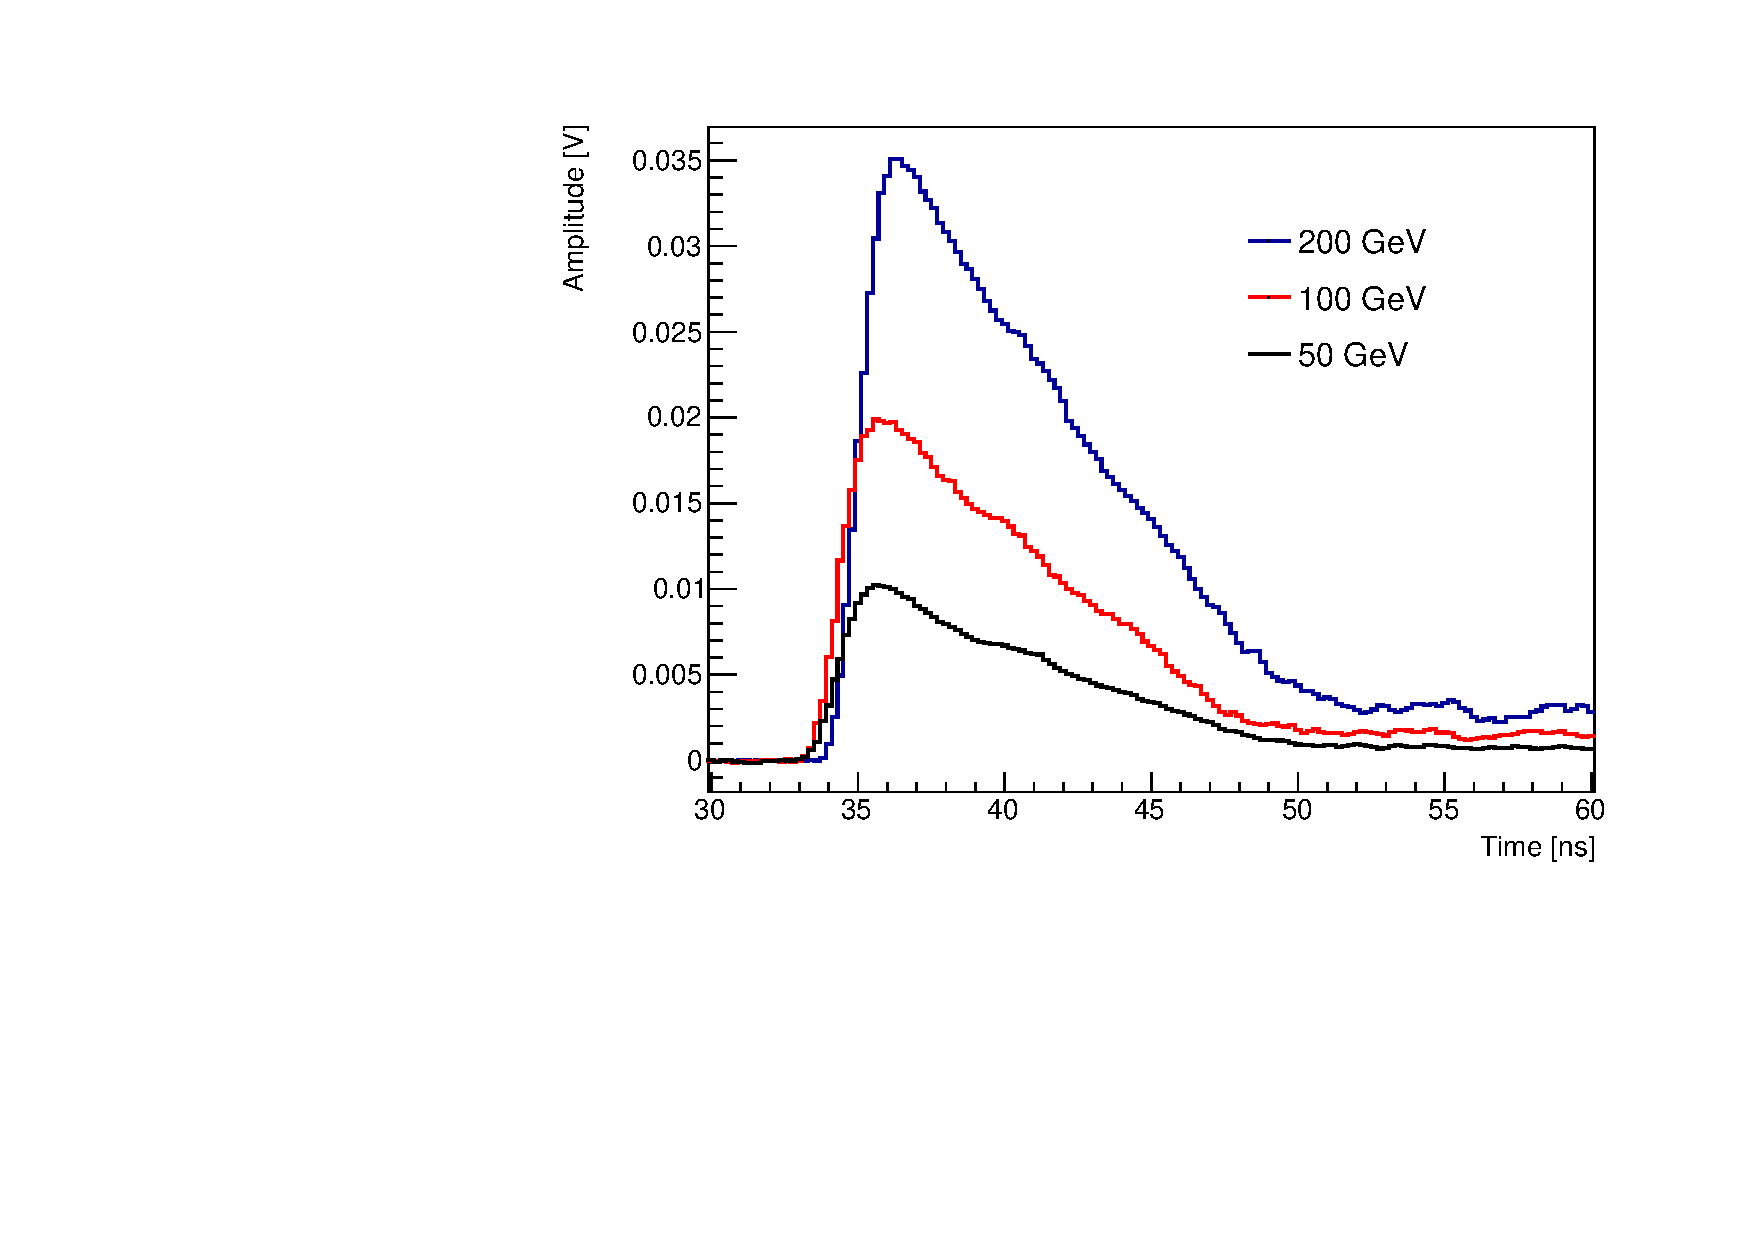
\includegraphics[width=0.49\textwidth]{figures/TypicalPulses_Zoom.pdf} 
\caption{Examples of signal pulses in the CdTe sensor for electrons with energies of $50$~GeV,
$100$~GeV, and $200$~GeV. Right: Zoom in of the example pulses.} 
\label{fig:Pulses} 
\end{figure} 

The total charge collected in each channel is obtained by computing the integral of the pulse
waveform. The time stamp for each signal is reconstructed by fitting the pulse waveform with
an appropriate functional form. For signal pulses from the MCP-PMT's, used as reference timers, 
we fit a gaussian function to a $1.5$~ns window around the peak of the pulse and extract the 
timestamp $t_{0}$ as the mean parameter of the gaussian function. For signal pulses from the
CdTe sensor, we fit a linear function to time sample points between $10\%$ and $60\%$ of the pulse
maximum and the timestamp $t_{1}$ is assigned as the time at which the fitted linear function
rises to $30\%$ of the pulse maximum. More details of the time stamp reconstruction can be
found in reference~\cite{Anderson:2015gha}.


Based on the results shown in Figure~\ref{fig:BeamSensorPosition}, we select events
for which the incident beam particle lies within the geometric area covered by the 
CdTe sensor. The region with X coordinate between $2.5$~mm and $13.5$~mm and
Y coordinate between $-8.0$~mm and $2.0$~mm is selected. We require that the 
signal in the reference MCP-PMT detector has an amplitude larger than $25$~mV. 
For data collected at the H2 beamline, the MCP-PMT detector is located behind
the absorbers and can disriminate between electrons that shower in the absorber
material and pions that do not. We require that the signal amplitude in the 
MCP-PMT detector is larger than $500$~mV to select a pure sample of electrons. For
data collected at the T9 beamline, the electron selection is performed using
the LYSO scintillating crystal placed behind the absorber material and the CdTe sensor,
as shown in Figure~\ref{fig:BeamSchematicDiagram}. The electromagnetic shower particles produce
scintillation light in the LYSO crystal and are read out by an MCP-PMT. We require that
the signal amplitude in the MCP-PMT coupled to the LYSO crystal is larger than $800$~mV
to select a sample of pure electrons. Furthermore, as the precision of the beam particle position 
measured by the wire chambers at the T9 beamline is relatively poor, we also require
large signals in the $1$~cm~$\times$~$1$~cm scintillator trigger counter, with
amplitude above $150$~mV, to constrain the beam to a smaller geometric region. 

